\documentclass{l3proj}

\usepackage{float}

\begin{document}
\title{Global Rugby Network FanZone (Web)}
\author{Ruxandra Bob \\
		Marios Constantinou \\
        Daniel Juranec \\
        Arnas Kapustinskas \\
        Andrew McCluskey}
\date{10 February 2017}
\maketitle
\begin{abstract}
Report on Team Project 3 coursework for Group V. The GRNFanzone is a
 fan engagement web application developed to interface with the Global Rugby
 Network's online platform. The project tried to utilise
 emerging technologies ranging from Angular to Firebase, and use
 cutting-edge methodologies, such as Behaviour Driven Development and Agile
 project management. This report covers some of the considerations taken
 during development and explains some of the benefits and disadvantages
 of the way the development team operated. The report will also the lessons
 the team learned over the course of the six months.
\end{abstract}
%% Comment out this line if you do not wish to give consent for your
%% work to be distributed in electronic format.
\educationalconsent
%TODO: Remove this later
\newpage
\tableofcontents
\newpage
%==============================================================================
\section{Introduction} %1-2 pages

This paper presents a case study of the project and software development process
 of Group V, which consists of five Software Engineersing students at the
 University of Glasgow, as part of the University's Team Project 3 course.

Our customers for the project were Global Rugby Network (GRN), who tasked us
 with creating a web application that would allow professional and amateur
 rugby clubs, teams, and players to interact with rugby fans. This social
 platform would then be integrated with the software that GRN already provides
 to rugby clubs. The end result is GRNFanZone, a fully functioning web application
 that allows people to follow their favourite clubs, see the latest posts
 made by them, find rugby matches happening near them, and much more.

The purpose of this document is to reflect on the achievements and challenges
 that arose during the development of this project. It also explores the concepts
 and methodologies touched upon in the concurrently running Professional Software
 Development (PSD) course, how we decided to implement them, and the effectiveness
 of our implementation.

The rest of the case study is structured as follows.

Section \ref{sec:background} presents the background of the case study
 discussed, describing the customer and project context, aims and
 objectives and project state at the time of writing.

Section \ref{sec:frontend} talks about the key technology used for the
 frontend implementation of the project. It contains an overview of the
 technology and justification for its usage in the project.

Section \ref{sec:backend} covers the key technologies used for the 
 backend development of the project. This section will also describe
 some of the difficulties faced by the team in this area.

Section \ref{sec:testing} %TODO

Section \ref{sec:cicd} discusses the Continuous Integration and Continuous
 Deployment techniques that were used in order to ensure higher quality
 of code and to continuously deliver new implementations. It also outlines
 challenges the team faced when using these techniques.

Section \ref{sec:planning} %TODO

Section \ref{sec:agile} %TODO

Section \ref{sec:conclusion} is the conclusion, where we evaluate our
 performance over the whole process, what has been learned from it and
 how this experience can benefit us in following professional software projects.


%==============================================================================
\section{Case Study Background} %4-5 pages
\label{sec:background}
Include details of

\subsection{Client Background}
\begin{itemize}
\item The customer organisation and background.
\end{itemize}

\subsection{Initial Objectives}
As mentioned above, our client's primary objective is to provide a platform that
 enables coaches to manage their teams.  The client noticed that there was a lack of
 fan engagement opportunities on their platform. As a result, our project motivation 
 and initial objective was to build an online social platform for rugby fans, who could
 be kept up to date with official information from teams.

GRNFanZone, was developed as a web application, and aims to provide users a way of
 interacting with their favourite clubs, teams and players, inside a user-friendly
 environment. The two initial target audiences included the profile-owners, and the
 profile-followers.

Profile-followers are the users who will be registering accounts with GRNFanzone to
 stay up-to-date with rugby news. As an initial step, followers sign in using Google or 
 Facebook accounts. After this, users are presented with a list of clubs, teams and players
 that they can choose to follow. Another requirement is letting profile-followers "unfollow"
 a currently followed entity. There is also the opportunity to get information about 
 upcoming fixtures.

Profile-owners represent the group of clubs, teams and players who have registered with
 GRN. These entities will not access the web application directly, but use their GRN account
 to provide information, which is subsequently pushed to the GRNFanzone and then presented
 to the profile-followers.

As a result, some could argue that our Project Motivation was to use technology, and help
rugby community generate additional engagement not only with potential followers and
supporters, but with sponsors as well.

In general terms, our aim was to use technology to encourage enagagement amongst the 
 rugby community - ranging from fans to sponsors.

\subsection{Summary}
\begin{itemize}
\item The final software was delivered for the customer.
\end{itemize}

%==============================================================================
\section{Frontend Technology Considerations} %1-3 pages
\label{sec:frontend}

At the start of the project, GRN chose to give us a set of technologies they
 wanted us to use. These included defining Angular 2 as our frontend framework.
 Angular is a framework maintained by google, which has been gaining popularity
 over the last 8 years\cite{angularjsoverview}. The framework uses typescript,
 a type safe flavour of javascript. Angular focuses on being portable, high performance
 and easy to write\cite{angular_features}. Many of the contributors to Angular are
 from Google, but the project is open source under the MIT license and anyone can
 commit to it\cite{angularjsoverview}. Angular is built on top of NodeJS, providing
 easy access to a wide range of external components.

Angular embeds code in html, and uses a "controller" to define component behaviour. This
 "component" object is the basis of most Angular development. Angular also tries
 to minimise the logic in controllers, by either abstracting it to other components
 or building "services" - shared libraries of code snippets. The final part of this 
 structure is a "module" which co-ordinates resource injection into controllers from one
 file. A project may have more than one module for it's subsections, but we stuck to
 one file. We made use of several services, and many components.

 % Pros and cons of ng-cli
Angular provides a CLI that makes it easy to start projects, and provides
 templates for components, services and modules. This provides the \texttt{ng init}
 command, which prepares a skeleton project in a matter of minutes.
 The basis of the project was generated in under a minute, which set up
 testing frameworks, a basic starter app and a \texttt{package.json} file for NPM.
 When generating a new component, a html template, CSS styles file, karma
 jasmine test file as well as the typescript controller. These were populated
 with template code to allow easy starts. This helped ensure we could get to
 the business logic of the component or service quickly, without wasting time.

  \begin{figure}[H]
\begin{center}
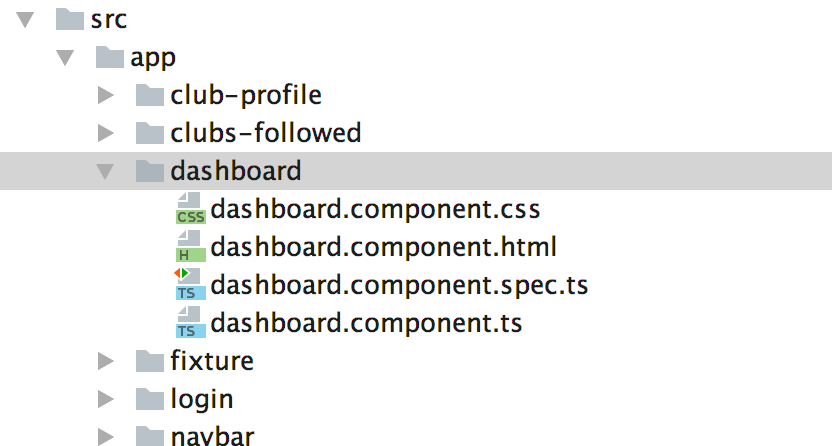
\includegraphics[width=7cm]{figures/frontend_components}
\end{center}
\caption{A selection of components used in the GRNFanzone}
\label{fig:frontend_components}
\end{figure}


 % Why we liked it (easy to maintain, works out the box, good documentation)
Angular 2 gave us a huge advantage when working on this project. Components provide
 an easy way of separating concerns, and reducing code duplication. Generating new
 code is easy with the CLI, and entire projects can be started and running
 in hours. The documentation for Angular is also excellent. Maintained by google,
 it is kept up-to-date with the regular releases Angular receives.

 % why we disliked it (steep learning curve)
The most significant barrier to using Angular was our own inexperience.
 Thus far, our formal education has not involved developing webapps in
 javascript based frameworks. Beyond this, typescript was new to every
 member of the team. This meant that there was a steep learning curve for
 the team to deal with and adapt to. This caused some issues early on,
 before we had a good grasp of how to use the actual features Angular
 provides.

 % How easy it was to test
One of Angular's benefits is that its developers have carefully
 considered testing. Software testing has long been an important
 aspect of software development, and this has only become more true
 in recent years \cite{tuteja2012testing}. The Angular CLI generates
 a functional karma file, which has been configured for Angular. The
 Angular CLI also provides an interface for running tests. Parameters
 range from single/constant runs of the test suite to enabling code
 coverage reporting. In spite of this, it was found to be very
 difficult to mock our services which used angularfire to generate
 good tests (please see section \ref{sec:testing} for more on this).

\begin{figure}[H]
\begin{center}
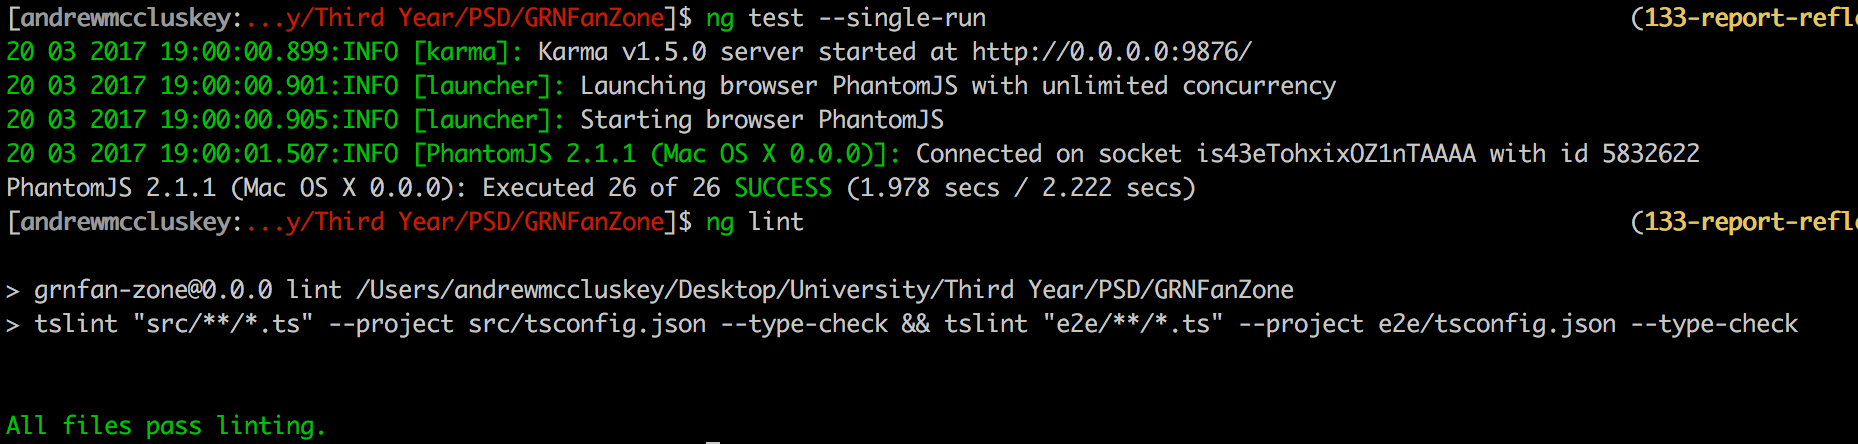
\includegraphics[width=11cm]{figures/frontend_ng_cli}
\end{center}
\caption{Using the Angular CLI to run tests and linting}
\label{fig:frontend_ng_cli}
\end{figure}


%==============================================================================
\section{Backend Technology Considerations} %1-3 pages
\label{sec:backend}

As with the frontend, our clients defined what technology they wanted the team
 to use for the backend of the project before we started development. We were
 tasked to use Firebase, which is a mobile and web application platform that
 was acquired by google in 2014. Its inital product was a NoSQL realtime database,
 however since then it has added a large range of features, including static
 hosting services, authentication and storage.

We started off by registering our project GRNFanZone on the Firebase website,
 which provided us access to the Firebase console, as well as an API key to
 initialise and access the database. Afterwards, we followed the documentation
 to implement authentication using Facebook and Google, which was an initial
 requirement for the project. Finally the team used Firebase's CLI to deploy
 the initial build using the provided static hosting service. This process
 was later refined and automated as part of our continuous deployment strategy
 (discussed in section \ref{sec:cicd}). Overall, the ease with which Firebase 
 allowed these features to be set up and implemented benefitted us greatly, 
 as it allowed us to concentrate on other parts of the project.

The main benefit of Firebase for the project was the realtime cloud-hosted
 NoSQL database. All of the data in the database is defined using JavaScript
 Object Notation (JSON). The database can be edited by using the editor
 in the online Firebase console, or by creating a JSON file and either deploying 
 it using the CLI, or importing it in the console. We used Globally Unique
 Identifiers (GUID) for main entity IDs, and divided our data into six main categories:
\begin{itemize}
\item
\textit{Users}, where every user would contain some personal information
 from social authentication, as well as clubs, teams and players that user
 follows.

\item
\textit{Posts}, containing the text and title of the post, the post
 author ID and some information about him, the comments and likes to
 that post, and a timestamp.

\item
\textit{Fixtures}, which contains the home and away team IDs and names,
 timestamps of fixture creation and kickoff, location, and the score if
 the fixture has already happened.

\item
\textit{Clubs}, where each club has their crest, name, description,
location, and the posts made by that club.

\item
\textit{Teams}, which, alongside the same identificatory information as
clubs, contains what club the team belongs to, the team's age group and
type, alongside posts made by the team.

\item
\textit{Players}, that has every players' name, age, bio, location and
 profile picture, as well as what team the player plays for and posts
 by them.

\end{itemize}
The angularfire2 package that was used to interact with the backend used
 observables to provide data, information was updated on the frontend in 
 realtime, even without refreshing the app. As the purpose of the web 
 application was to provide a social platform for rugby fans, all connected 
 users being synced to the database made for a much natural and interactive 
 user experience.

\begin{figure}[H]
\begin{center}
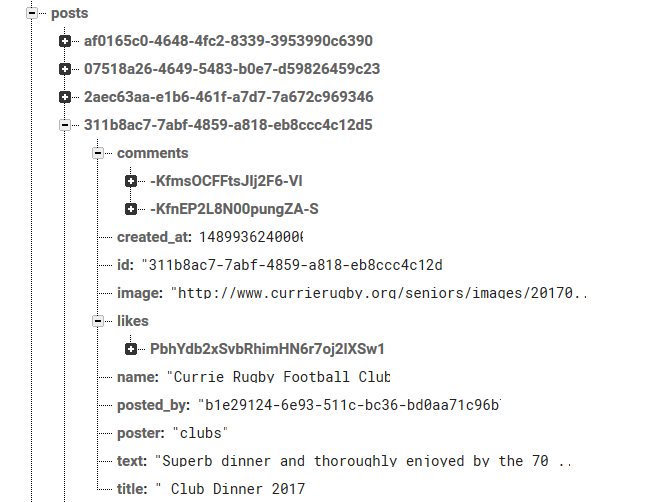
\includegraphics[width=11cm]{figures/backend_dbexample}
\end{center}
\caption{A snippet of the JSON used as the example database for GRN FanZone}
\label{fig:backend_dbexample}
\end{figure}


Firebase did not, however, come without its drawbacks. As usage of NoSQL
 databases has only recently become more prevalent, none of the team members
 had previously had experience of using or modelling data for one. Perhaps
 the biggest issue that arose while getting acquainted to using Firebase, was
 changing our relational database data modelling mentality to one that would work
 well with a NoSQL database. For example, duplicated data, which is considered
 undesireable in an SQL database, was necessary for us to be able to retrieve
 infomation about posts efficiently. It also meant that we had more limited
 functionality when it came to querying the database.

Another big issue was identified later on into the project. We used the
 Angularfire2 module to interface between Firebase and Angular2, which meant
 that all of our calls to the database had to be in the form of subscriptions
 to certain keys. As the application grew in complexity, more and more 
 subscriptions had to be made, due to which there arose some race conditions 
 concerning the load order of the data and issues where retrieved data would 
 be needlessly reloaded. Fixing these problems was very frustrating and took 
 up a lot of time that could have been spent implementing new features.

%==============================================================================
\section{Testing Considerations} %1-3 pages
\label{sec:testing}

% Describe BDD
Behaviour Driven Development is a development methodology where the development team
 first describes use cases for a feature, then writes tests for it, and lastly
 develops the code for the feature. The team decided to use BDD as it comes
 reccomended by the Agile Alliance \cite{agilealliance_bdd}. Another reason
 is that the angular CLI sets up a Karma Jasmine testing set up by default.
 BDD is credited with helping to develop easily documented code - for example,
 by making test cases into natural language sentences (see figure
 \ref{fig:testing_failed_test}), it becomes easier for human developers to
 understand what it tests, and why it is being tested \cite{north2006bdd}.

 \begin{figure}
\begin{center}
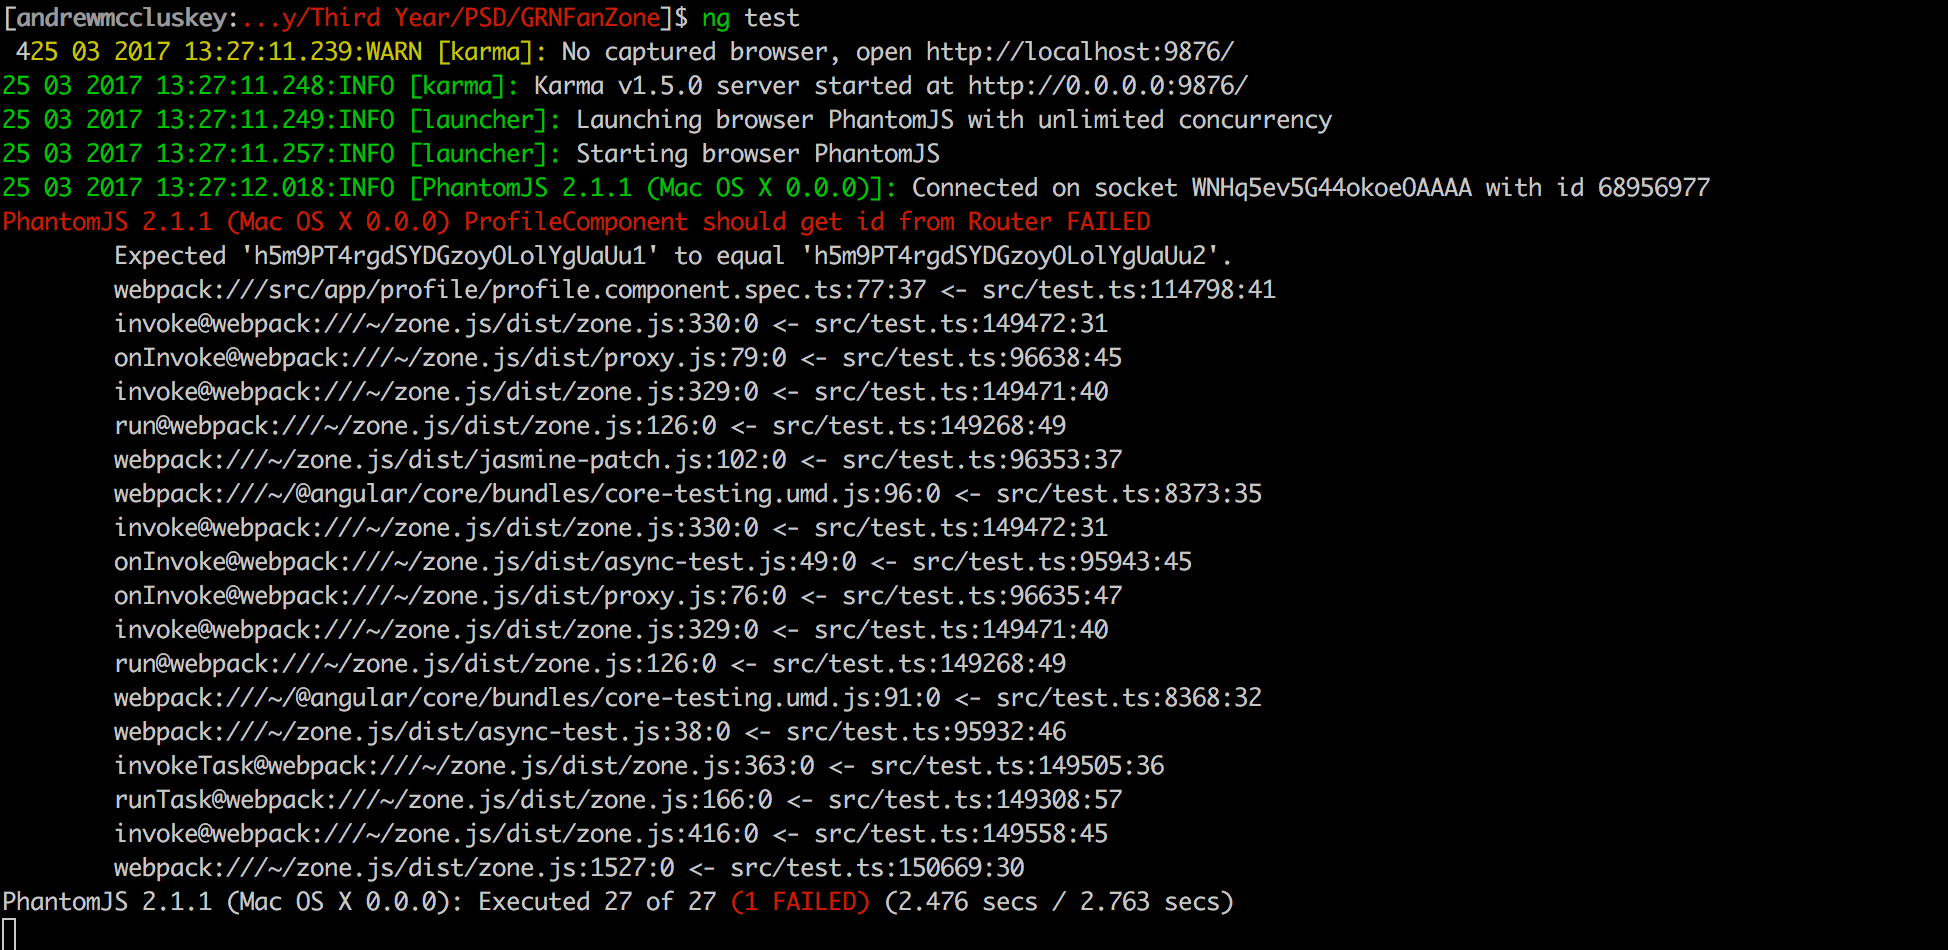
\includegraphics[width=11cm]{figures/testing_failed_test}
\end{center}
\caption{A failed test gives a human-readable failure message}
\label{fig:testing_failed_test}
\end{figure}

% Describe Karma and Jasmine testing with Angular2
The Angular 2 CLI sets up a Karma Jasmine configuration to run tests on
 the typescript in the project. Karma is a test runner for javascript
 that is platform agonostic and allows testing over different devices
 and browsers\cite{jina2013javascript}. Jasmine is a testing framework 
 that aims to be as readable as possible - one of the key features of 
 the BDD approach we wanted to adopt. Initially, we tried to use Mocha, 
 another testing framework which is targeted at Test Driven Development,
 however integrating it was difficult and was taking too long to set up, 
 so we decided to move from TDD to BDD and just use Jasmine. One of the 
 benefits this brought was the wealth of documentation and examples 
 across the internet of using Karma with Jasmine on Angular code.

% Describe how it was done well
% mention test coverage
By the end of the project, a number of tests had been incorporated into the 
 project. These tried to cover edge cases and a variety of conditions the GRNFanzone 
 could face in the wild. Our code coverage - a metric which enumerates what 
 proportion of the code is tested - tended to stay fairly high. We have exact 
 figures due to our Continuous Integration, which ran the tests every time a 
 commit was pushed(section \ref{sec:cicd}), though we did not place any constraints 
 on a minimum coverage value. Typically, the coverage ranged from 80\% to 60\%. 
 Towards the end of the project, the value was just over 75\%. This was 
 representative of just under 40 tests written. To increase transparency 
 across the project, we displayed values for our test coverage on dev and 
 master in the readme, using icons provided by Gitlab (see figure 
 \ref{fig:cicd_coverage_buttons}.

 The code coverage metrics also provided a file-by-file breakdown of where
 coverage was high or low. This proved to be helpful when choosing
 where to focus our effort - there's no point in writing tests for
 well-tested code, it makes much more sense to write new tests for the
 code that is less well tested. See figure \ref{fig:testing_coverage_metrics}
 for an example of the html display.

% Difficulties we faced
% reference common pitfall from agile alliance of being a big jump from tdd and hard for noobs
% Struggles with angularfire2
% struggles with @input components
Testing was not always easy. For example, getting into a habit of writing tests
 proved difficult for the team, showing that working in a development team on a
 complicated project is very different to working on individual projects. The
 Agile Alliance warns that "BDD requires familiarity with a greater range of
 concepts than TDD does, and it seems difficult to recommend a novice programmer
 should first learn BDD without prior exposure to TDD concepts"
 \cite{agilealliance_bdd}. This turned out to be a significant difficulty for
 our team. This demonstrated to us first hand that it is important to choose where
 in the project a team should focus their learning time, and that too much new technology
 can stretch a team to the point where the effort spent to learn new things 
 overtakes that spent on features.

Another struggle was getting tests to run. Due to the interconnectivity of
 Angular components, a complex data flow has to be replicated. For example,
 components that use the \texttt{@input()} tag to receive data don't have a
 trivial way of faking this. This means that the data flow there becomes
 difficult to test accurately. Had this not been such an issue, the post
 component would have been much easier to test - currently, it has the worst
 code coverage in the project.

There were also issues when testing backend connections. Whilst it is
 allegedly possible, the team did not find a way of mocking Angularfire2, the
 service which provides an interface between Angular and Firebase. This meant
 that tests would affect the production database, something which could not be
 allowed. As a result, calls made to angularfire were not tested, despite the
 fact that they constituted a significant amount of our business logic.

Overall, the team's testing methodologies were too optimistic. We assumed that
 we could make a large jump to an unfamiliar methodology, whilst also learning
 to write new tests. Another of the mistakes we made was putting testing aside
 and instead trying to get features out. This resulted in a code base that did
 not have the test coverage we desired, but also gave us a large task in writing
 the tests after the fact. This proved more difficult than writing them as we
 went along.

 \begin{figure}
\begin{center}
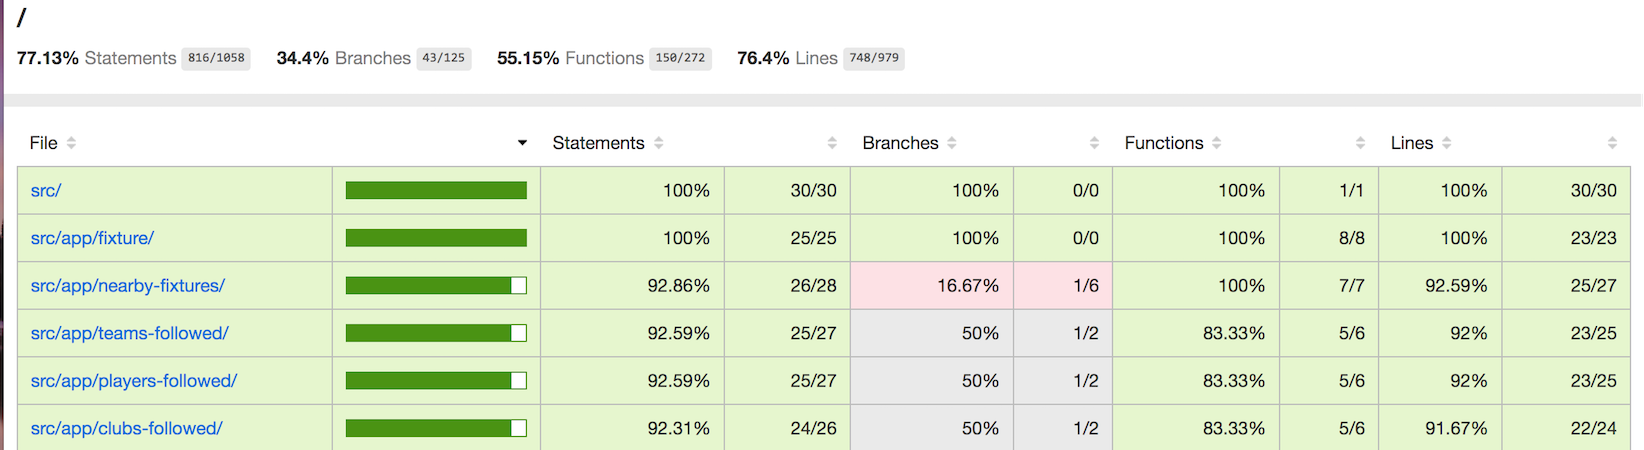
\includegraphics[width=11cm]{figures/testing_coverage_metrics}
\end{center}
\caption{The html report on code coverage}
\label{fig:testing_coverage_metrics}
\end{figure}

%==============================================================================
\section{Continuous Integration and Deployment} %1-3 pages
\label{sec:cicd}

The project used a multitude of Continuous Integration (CI) and Continuous
 Deployment (sometimes Delivery) (CD) techniques. A CI server's purpose "is to check the code
 repository for changes, check out the code if it spots any [changes], and run a
 list of commands to trigger the build."\cite{meyer2014continuous} A build is "ideally more than just
 compiling - it should also include a thorough test suite to help verify that the code
 still works with every change."\cite{meyer2014continuous} This gives a development
 team a quick, automated way of checking their code works, follows a style guide and
 doesn't break any other work.

One of the key concepts of CI is often phrased as: "Commit Daily,
 Commit Often"\cite{meyer2014continuous}. For our project, this was sometimes a struggle.
 This was due to a small number of factors, which boiled down to: "We don't work on the project
 every day", and "I'm not used to git". There was little we could do to remedy the former issue -
 all we could do was commit often \textit{whilst we worked on the project}. The gitflow
 branching system we used in the VCS (see section \ref{sec:planning}) was unfamiliar to several
 members of the team, and it took time for everyone to become accustomed to the system. As the
 project progressed however, more builds were made, more commits pushed, and more bugs found.

Another hurdle at which we fell was getting into the habit of writing tests for our code. I shall
 mention this briefly here, but for more details please see section \ref{sec:testing}. In Fowler's
 2006 paper on CI, he says: "Imperfect tests, run frequently, are much better than perfect tests
 that are never written at all."\cite{fowler2006continuous}

Continuous Deployment is the practice of continually deploying working builds to production
 as often as possible. It adheres to the Agile principles of:
 \begin{itemize}
 \item
 Our highest priority is to satisfy the customer
 through early and continuous delivery
 of valuable software. \cite{agileprinciples}
 \item
 Deliver working software frequently, from a
 couple of weeks to a couple of months, with a
 preference to the shorter timescale. \cite{agileprinciples}
 \end{itemize}
 In our project, as soon as a new feature is merged into the dev branch,
 tests are run, and then the changes are deployed to a staging server, hosted by firebase. Similarly,
 as soon as dev is merged into master, master is pushed to our production server, also hosted by Firebase.
 The dev branch was typically merged into master once a week, allowing time for any changes to be made
 to features that weren't quite perfect, and to iron out any bugs that were found after time in dev.

Our CI and CD was operated using Gitlab's integrated CI system. This uses docker to
 run a set of instructions defined in the 'gitlab-ci.yml' file.  Instructions are
 separated into tasks. Tasks belong to stages - in our project, these were
 "test" and "deploy". The tasks are run as builds within a pipeline. The docker instances were
 in some cases hosted for free by Gitlab (sponsored by a cloud company). In other cases,
 builds were run on team computers. A common upper limit for build time is quoted as
 10 minutes\cite{fowler2006continuous} - ours typically ranged from 5-15 minutes, with some exceptions that were
 typically waiting on the gitlab CI runners to free up. The single largest time-drain was
 running \texttt{npm install} every time docker span up a new instance. Running builds
 typically took under a minute after this.

 \begin{figure}[H]
\begin{center}
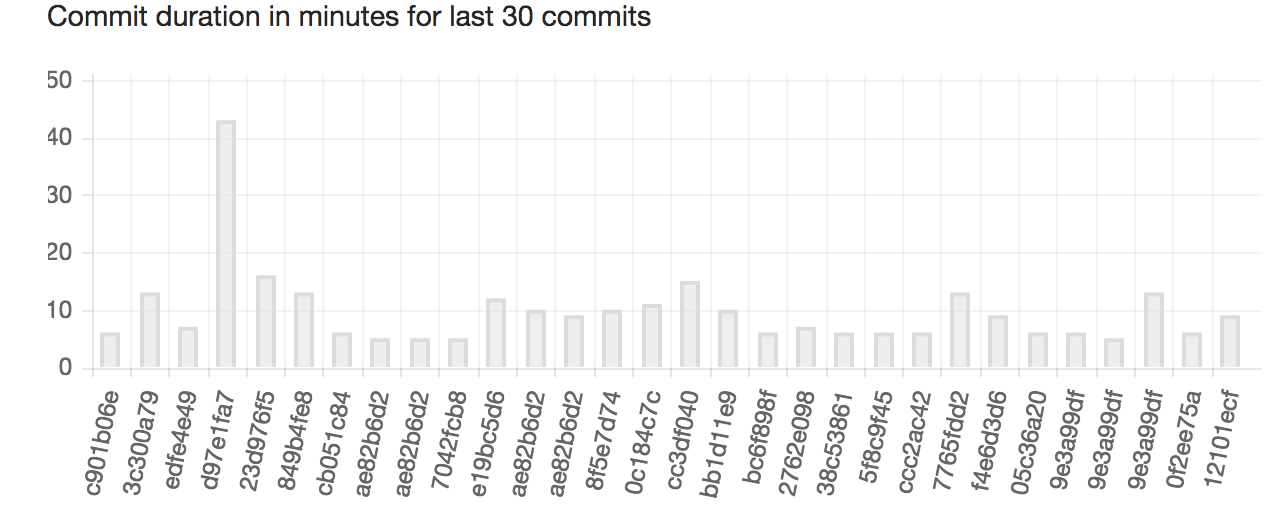
\includegraphics[width=9cm]{figures/cicd_build_duration}
\end{center}
\caption{Build Duration for last 30 commits from 21:28 on 19/03/2017}
\label{fig:cicd_build_duration}
\end{figure}


% Describe Linting task
The first task used by the project's "test" stage ran a series of lint checks over the
 project's source code. Linting involves performing static analysis on code to detect bugs
 or violations of a style guide. These kind of checks are also performed by compilers and
 so on. These issues can range from missing semicolons, to using a mix of
 double and single quotes, to whether a function is never called. The task tested CSS,
 JSON, typescript, javascript,  HTML and LESS. Whilst this was often annoying, these tests
 did help maintain a higher quality of code in the codebase. As our policy was to not allow a
 merge to dev take place if a branch was not passing tests, we had a method of
 enforcing that the standards we defined were upheld.

% Describe testing task
The second task ran the project's tests. Again, this task had to complete successfully in
 order for a branch to be merged into dev. This stage also generated coverage reports which
 were used to give the team an indication of how well our code was tested.

 \begin{figure}[H]
\begin{center}
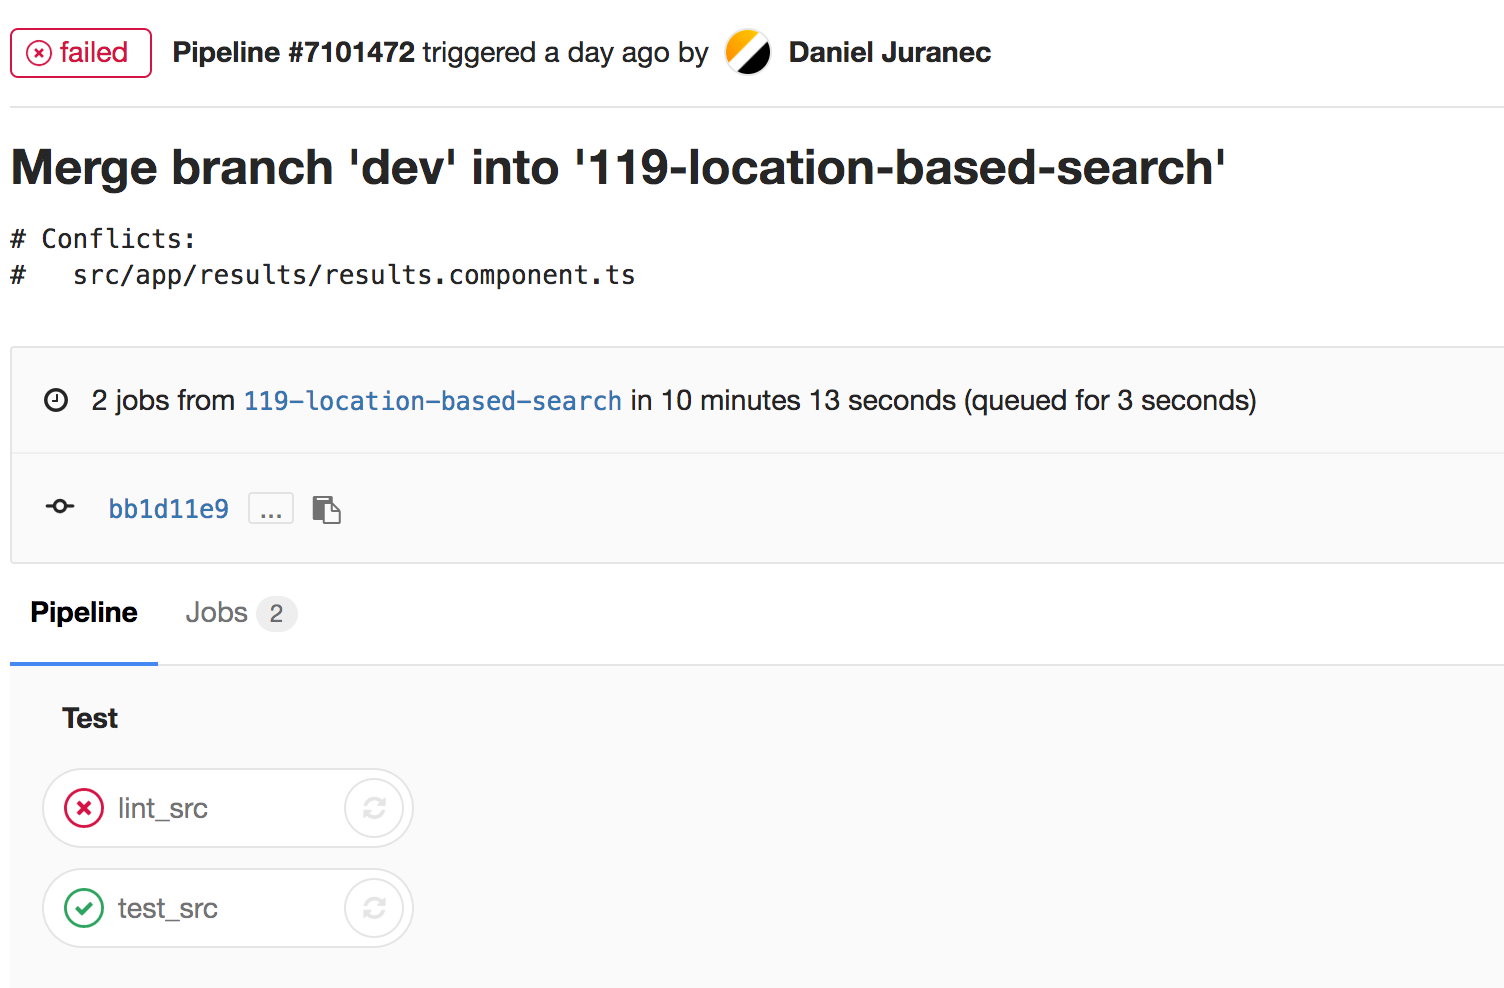
\includegraphics[width=9cm]{figures/cicd_failed_pipeline}
\end{center}
\caption{Example of a failed pipeline in GitLab}
\label{fig:cicd_failed_pipeline}
\end{figure}


% Considered combining test tasks
Merging these two tasks was considered, but left aside for now. The tasks take 5-10 minutes
 each to run, and are run in parallel. The downside of this separation is the fact that \texttt{npm install}
 is run twice. However, by leaving the tasks separate, we get a quicker, clearer indication
 of which part of the stage failed - actual functionality, or a style issue.

 \begin{figure}
\begin{center}
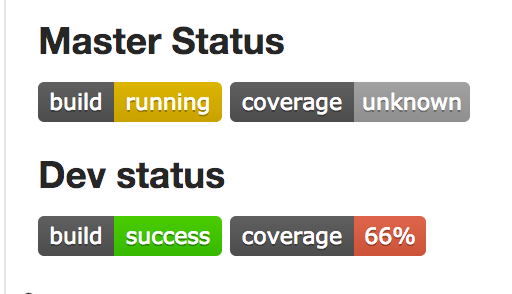
\includegraphics[width=4cm]{figures/cicd_coverage_buttons}
\end{center}
\caption{The buttons used to display pipeline status and test coverage}
\label{fig:cicd_coverage_buttons}
\end{figure}

% Describe deployment tasks
The continuous deployment tasks were both essentially the same, but related to which branch was being
 committed to. As both dev and master can only be merged into instead of committed to, these tasks can
 be run only on merge commits to dev or master. The tasks run tests (to allow coverage reports for the branches)
 and then deploy to our live servers. The dev branch deploys to the staging zone, and
 master to our production site.

The fact that this is automated helps encourage rapid deployment, as the steps take some time, and are
 boring for people to do. This methodology takes out the human steps, and means that the development team
 can focus on development. These rapid deployments also help by making it easy for the team to demonstrate
 and generate feedback from the public. This also allowed the client to continuously check our progress and
 give us feedback.


% consider how it helped us and how it could have been improved
The CI and CD processes helped us by keeping our code of high quality, preventing broken commits and reducing
 manual time spent doing menial tasks. However, it took a fairly large period of time to get working and to
 optimise into time chunks that were consistent with the goal of 10 minutes. It is arguable that the time
 could have been better spent working on the actual project itself. As a counterpoint to this, it could be
 argued that the CI and CD has saved the development team time in fixing bugs later on, and by ensuring code is more
 readable, reducing time wasted understanding the code.

 %==============================================================================
\section{Project Planning} %1-3 pages
\label{sec:planning}

After the project allocation day, GRN have sent us a project brief containing
 more details about the project itself, as well as a list of functional
 requirements that the final product was expected to meet. The first
 task we needed to complete was a detailed requirements document, that would
 contain non-functional and any additional functional requirements. It was
 decided that the focus of the first month would be allocated to finalizing
 the document, in order to assure that the client approved of the direction
 the team decided to take in working on the project.

As part of the requirements gathering process, the team developed four personas
 and an epic user story of how they envisioned the project being used. This was followed by
 writing down user stories centered around the following entities: team manager,
 sponsor, player, club supporter, rugby fan and international rugby fan. Doing
 this eased the process of identifying useful requirements and helped the team
 visualize what the final product should be offering potential users.

After the initial requirements were outlined, the team followed by designing
 wireframes of the web application. Initially, each team member delivered a
 pencil-drawn sketch of each expected application screen. Afterwards, the
 best design from each wireframe were merged into the main wireframes, drawn
 using draw.io. GRN warned us that the main wireframes would not offer useful
 guidance when thinking how the application should transition to a mobile format,
 so the team repeated the process to generate mobile wireframes.

Over the weeks dedicated to producing the requirements document, the team
 kept close contact with GRN, who have repeatedly offered helpful feedback
 and guidance regarding how the team can meet their expectations of the
 final product. This was in the form of a weekly progress email, and a monthly
 physical meeting, giving us some understanding of what the client found
 to be of most importance, and it helped us in the next stage in our
 project, which was prioritising the features of the application and separating
 them into achievable goals for each iteration.

There were several aspects to be taken into consideration while deciding
 on a concrete structure of the development process. We had to consider
 our lack of experience with the technologies to be used and the fact
 that the available time to work on the project would vary as the academic
 year progressed. Another thing to consider was the fact that due to the
 agile methodology we decided to follow, at the end of each iteration, the
 product needed to be functional. Thus, it was decided to settle on having
 smaller, more easily achievable goals in the beginning, which would
 incrementally become more complex as advanced. In the end, we settled
 on seven iterations, excluding the initial one focused on the requirements
 document.

The goals for each iteration become increasingly challenging, based on the
 expectation that the first one or two iterations would offer all team
 members some hands on experience with both Angular2 and Firebase. The
 goals for each iteration were the following: 
\begin{itemize}
\item First iteration - login and sign up
\item Second iteration - dashboard and followed pages
\item Third iteration - post creation and management
\item Fourth iteration - view and edit profile, posts on comments
\item Fifth iteration - search for teams/clubs/players or fixtures
\item Sixth iteration - translation and additional tasks
\item seventh iteration - additional features, refinement, documentation
\end{itemize} 

\begin{figure}[H]
\begin{center}
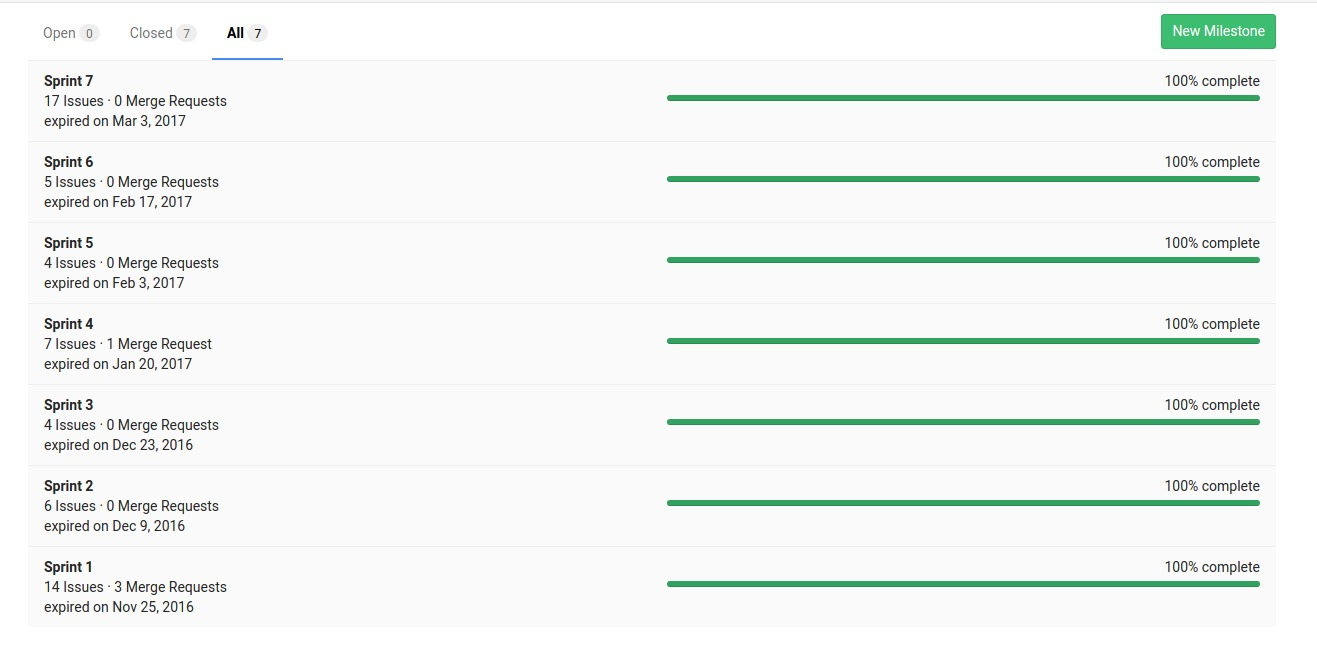
\includegraphics[width=15cm]{figures/planning_milestones}
\end{center}
\caption{Project milestones on GitLab}
\label{fig:planning_milestones}
\end{figure}


Gitlab allowed us to create project milestones. Each of them had a number
 of issues associated with it, the issues consisting of the goals for the
 respective iteration split into several multiple smaller issues. The deadline
 of each iteration would also appear on each issues, becoming bright red as the
 date came nearer, in order to alert the person assigned to the task.

Throughout the project, our process was modified and improved by having team
 retrospectives around the end of each iteration. The format of the retrospectives
 consisted of every team member going through what they thought went good in
 our past iteration, what they thought went bad and what ideas they have to
 improve our workflow in future iterations. All these were discussed within
 the team and what the majority considered useful ideas were then included
 in the further development. The main points of each retrospective are
 documented on the wiki page of the project, which can be found on Gitlab.

%==============================================================================
\section{Agile Methodology} %1-3 pages
\label{sec:agile}

% short description of agile development

Agile software development consists of a set of practices and methods derived
 from the principles described in the Agile Manifesto. Agile enforces a strong
 collaboration between the development team and the business stakeholders,
 self-organizing teams and frequent delivery of functioning
 software\cite{agile_overview}.

As agile development was highly recommended as part of our software development
 process, in the initial team meetings, we decided to use the Scrum
 methodology.

 % short description of SCRUM
 Scrum is an agile framework originally formalised for software development
 projects. Scrum defines several major roles within the framework: the product
 owner, the scrum master, the development team and the customer. The product 
 owner should maintain communication with the stakeholders and create a prioritized 
 list goals to be achieved. The scrum master keeps the team focused and leads team 
 meetings.\cite{scrum_overview}

 % our agile development
 Within our team, Andrew was the product owner and Ruxandra was the scrum master.
  After the first few team meetings, where the focus was on finalizing the initial
  requirements gathering, the focus was shifted to dividing the prioritised
  expected features. As a result of discussions between the product owner and
  the rest of the team, it was decided to split the work into seven sprints,
  each of them lasting two weeks. One sprint would end on Friday and the next
  one would start the following Monday (Figure \ref{fig:agile_gantt}).


 It was decided that instead of daily scrums, the team would have two weekly
  meetings, one on Wednesdays, during the software development lab, and one on
  Fridays. The format of the meetings included everyone describing what they've
  worked on since the previous meeting and the work they plan on completing
  until the next meeting. Each team member also discussed any difficulties
  they encountered, how they overcame them or whether they feel that they
  need help with certain issues.

 The scrum master was tasked with closely observing these meetings. They had
  to determine whether the team could handle the workload of the respective
  sprint, if everyone in the team had something to work on and how to efficiently
  assign members to assist those who need help with something. The scrum
  master would also take into consideration any complaints or suggestions from
  the rest of the team, as well as initiate team retrospectives at the end of
  each sprint.

 As the project progressed, our scrum process underwent a few changes. Once
 the desired goals and the predicted timelines were better defined, it was
 decided that one meeting during the PSD lab would be sufficient, with any
 additional meetings to be arranged if deemed necessary. Meanwhile, the team
 would communicate daily through a group chat on Facebook messenger, in order
 to keep everyone updated with the general progress.

Towards the end of the first semester, our sprints needed quite a few
 adjustments, due to the increase in additional assignments from other
 courses, that everyone in the team had to complete. There was also a
 slight halt in communication during the winter break, as team members
 went home for the holidays. However, the additional time left at the
 end of our initial schedule allowed us to maintain the initial seven
 sprints and just shift everything by a few weeks.

As we became more comfortable working as a team and since at that
 point everyone was comfortable with the new technologies, team
 meetings became less structured and less formal. Along the way,
 the meetings became open discussions, while still making sure
 everyone is kept up to date. At the beginning of the second
 semester, our scrum framework transitioned into a less clearly
 defined agile framework, which still followed the main principles
 of the methodology. Sprints became of variable length (between
 one and three weeks) rather than a constant two weeks.

 \begin{figure}
\begin{center}
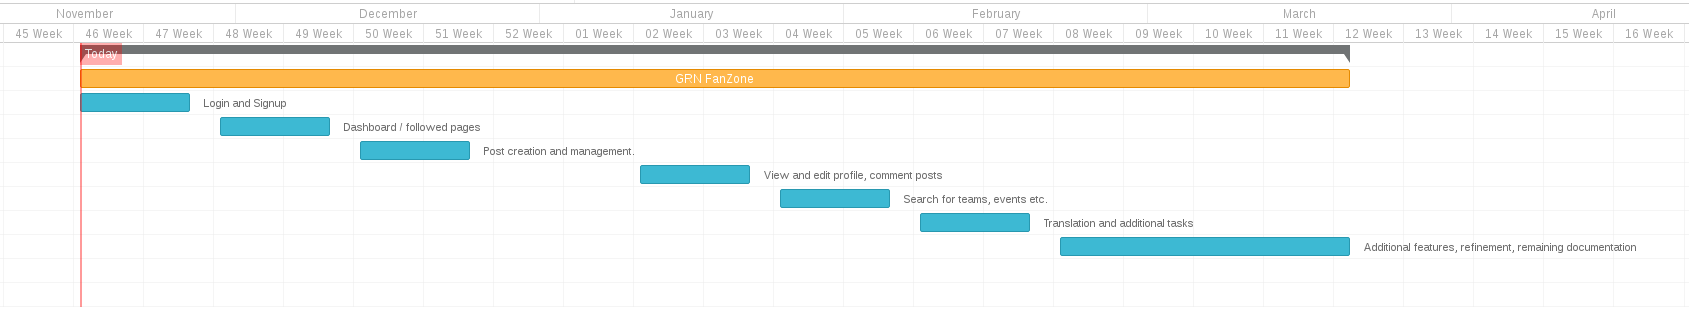
\includegraphics[width=15cm]{figures/agile_gantt}
\end{center}
\caption{Gantt Chart for Development Process}
\label{fig:agile_gantt}
\end{figure}


At the beginning of the development process, the product owner split
 every goal into separate small issues. Over the course of the project,
 these were refined and split further. The members of the team were
 also encouraged to make small commits as often as possible and only
 merge one small issue at a time in a separate development branch, in order
 to avoid disrupting someone else's work by generating conflicts.
 Every merge request needed to be approved by at least one other
 team member following a code review, in order to maintain the quality 
 of the product. These code reviews helped us to spot obvious mistakes,
 and to improve team understanding of how components worked.

At the end of each sprint, the product was fully or almost fully
 functional with respect to the features that needed to be completed
 up to that point. The end of most sprints coincided with the customer
 meetings. Thus, we were able to receive almost immediate feedback
 from both GRN and supervisors. This also offered us the opportunity
 to make additional improvements in the short time left between sprints.

To maintain the close communication with our client, as dictated by
 the agile methodology, the product owner would communicate weekly
 updates by email. The team was also in close contact with the
 development team of our client company, which was available
 for questions and pointed us towards useful resources. This
 was helpful in assuring that our version of the product would
 be as close as possible to the expectations of GRN, with respect
 to both design and implementation.

%==============================================================================
\newpage
\section{Reflection on Change Management Methods}
\label{sec:changemgmt}

At the very start of the project, we used a shared Google Docs folder to exchange initial ideas, such as user stories, wireframes, etc. Of course, when we had to start coding, some kind of version control repository had to be selected, and our choice landed on GitLab. The main attracting features of GitLab for us were the support for Git, which we all were familiar with at this point, and issue tracking, which enabled us to submit feature requests and bug reports with ease.

After we gathered the requirements for the project and defined the general development timeline, the issue tracker had to be filled in. GitLab allowed us to firstly create the sprints (with the possibility of assigning a deadline to each of them), and afterwards the feature requests could be assigned to a particular sprint. Additional attributes, such as assignee (the person responsible for resolving the issue), labels (feature, customer request, hotfix, non-essential, etc.), weight (1-10; decided during team meetings and retrospectives) could also be added, streamlining the development process.

For our branching model we selected one called Gitflow. \cite{gitflow} At its core, there are two main branches - dev and master. The master branch is the production-ready branch, and it reflects the state of the latest production release. Meanwhile, the dev branch reflects the state of our latest development efforts. We usually merged the changes from dev into master once a week to ensure the least amount of bugs possible, as most of the testing was done even before merging to the dev branch.

\begin{figure}[H]
\begin{center}
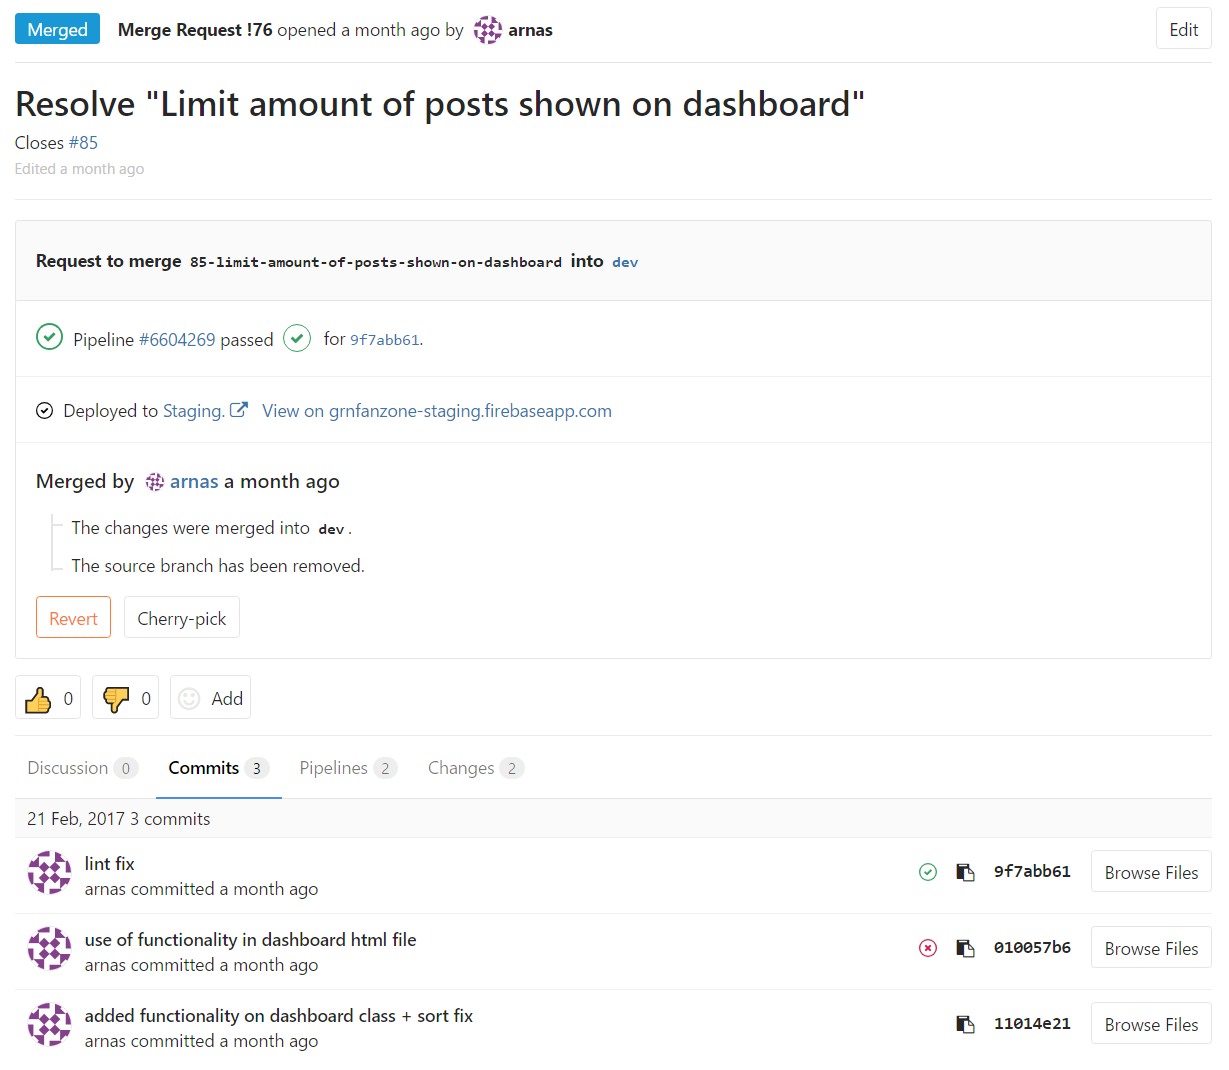
\includegraphics[width=11cm]{figures/changemgmt_merge_request}
\end{center}
\caption{Example of an approved merge request}
\label{fig:changemgmt_merge_request}
\end{figure}

In the Gitflow model, dev by itself does not allow any commits. therefore all the development has to be done in separate branches, called feature branches. For each issue in the issue tracker, its assignee created a new branch, and went on coding in that branch. We encouraged every team member to commit often, as it let us follow the development process better; to add to that, the testing of every commit, powered by our continuous integration system, enabled us to catch bugs early on. After the development of the feature was done, the assignee submitted a merge request for the feature branch to be merged into dev. It first had to be approved by any other team member, after he performed a code review. Code reviews allowed us to find mistakes in the source code not noticed by the developer, and therefore improve the quality of our project. If any mistakes were found, the reviewer could add some comments to the merge request, explaining what could be improved. Another thing which could prevent the merge request was merge conflicts. They occured if Git could not figure out on its own which lines of the source code to add, keep or remove, in case that files in dev and in feature branch differed greatly. It was on the assignee to resolve the merge conflicts. In the end, if CI tests passed, the merge requests were resolved, and the code reviews were performed, the merge request could be accepted. It resulted in the issue being closed, the new code being merged into the dev branch, and the feature branch being removed, so as not to clutter the repository with unnecessary files.

Encountering some issues with the workflow of GitLab was unavoidable. For example, if a feature branch was not being worked on for some time, it was getting behind dev, resulting in a lot of merge conflicts. The solution was either to resolve all of those manually, or, if there was not much progress done on the feature branch - simply remove it and start over. Code reviews were not always performed carefully (or not at all, during crunch time), so problems were often encountered even on the dev branch. On the other hand, the issue tracker did not cause any major issues; its level of convenience and robustness helped us get on the issues quickly, submit bug reports when encountered, and generally stay on top of the things.
    

%==============================================================================
\section{Conclusions} %1-2 pages
\label{sec:conclusion}

Explain the wider lessons that you learned about software engineering,
based on the specific issues discussed in previous sections.  Reflect
on the extent to which these lessons could be generalised to other
types of software project.  Relate the wider lessons to others
reported in case studies in the software engineering literature.

% Main Points: 
% Co-ordinating teams
% Wasting time on setup instead of features
% Compromising on systems
% Client requirements affecting our choices
% Learning new technology is part of the industry

This software project was a valuable learning experience. Each and every one of
 us learned new technologies, in addition to a much improved understanding
 of what working in a team over a long period of time involves. These lessons
 included: teamwork, organisation, time management and communication.
 
One of the biggest issues we first faced was co-ordinating ourselves as a 
 new team of strangers. By using icebreaker excercises to get to know 
 one another, and discussing our strengths and weaknesses, we got to 
 understand where each member of the team was comfortable working. There
 were occasionally difficulties in getting everyone to meetings and ensuring
 work was done on time, but by communicating well, we managed to share
 meeting information and helping each other out on difficult issues.
 
We also discovered that whilst the project's architecture is important, 
 it is also important to remain focussed on the actual product. We 
 spent a considerable amount of time at the start of the project setting 
 up the VCS, branching strategy, Gitlab and CI configuration. Whilst these
 were all valuable to the project, it would have been worth taking a step
 back and asking "is this the best thing for the customer?". Finding a balance
 is important.
 
As GRN already uses certain technologies (such as Angular 2 and Firebase),
 we were asked to also use them in order to ensure compatibility. GRN also
 gave us feedback that differed from what we expected, resulting in us 
 having to change our mindsets (particularly at the start of the year,
 before the team developed a clear vision for it). This taught us that 
 whilst you may want to do things in your own way, the client is ultimately
 the decision-maker for many choices. By having regular contact with them
 allowed us to get feedback quickly and reduced the risk of a feature that
 would have to be completly scrapped.
 
Many of of these technologies were new to the team (and to the industry), 
 which meant that we had to learn them in a short period of time. This 
 ate into development time, but was also necessary to fulfil the client's 
 needs. Learning these new technologies was interesting and challenging,
 but also came at the cost of time we could have spent on developing 
 features, and resulted in bugs that would not have existed if a more 
 familiar framework had been used. Ultimately, learning to use new, different
 technologies is a fundamental part of being active in computer science,
 and the ablity to aapt quickly to new ways of thinking will serve us well
 should we choose to go into industry.
 
The project gave us a chance to experience the world of software development
 first hand. We learnt about pitfalls to avoid in the future, but also how 
 to work well in a team and put our education into practice. This experience
 will certainly be of great use to us in the future, from the technologies we
 learnt, to the mistakes we made, to the late nights coding before client meetings.

%==============================================================================
\newpage
\bibliographystyle{plain} %1-2 pages
\bibliography{dissertation}
\end{document}
\grid
